\renewcommand{\leftmark}{MISE EN OEUVRE}
\chapter{Mise en oeuvre}\label{chap:work}
    Ce chapitre décrit la mise en oeuvre de l'architecture définie dans le
    chapitre~\ref{chap:archi}.
    % on fait d'abord python puis c

    Deux implémentations sont réalisées. Celle de la racine LoRa en Python 3.8.10 et celle de la racine RPL avec la version \texttt{Contiki-NG-develop/v4.7\\-18-ga3f6b04c5} de Contiki.

    Chaque implémentation est divisée en trois parties analogues aux couches physique, liaison et 
    réseau du modèle OSI. La chouche physique contient notamment un driver permettant d'abstraire 
    les communications UART avec le RN2483, rendant sont utilisation plus facile. La couche liaison 
    implémente le protocole LoRaMAC, et la couche réseau sert d'interface permettant d'envoyer ou 
    de recevoir des paquets IPv6.
\section{Racine LoRa}\label{sec:work-lora-root}
\renewcommand{\rightmark}{Trames LoRaMac}

    Le RN2483 est interfacé à l'ordinateur de développement via un bridge USB-UART.

    L'implémentation se présente sous forme d'un package python qui donne accès à une variable 
    \texttt{NETWORK\_STACK} qui fait référence à une instance de la classe \texttt{NetworkStack} et permet d'accèder aux trois 
    différentes couches, l'adresse LoRaMAC du noeud, son adresse IPv6 issue de la conversion de son 
    adresse LoRaMAC ainsi que trois fonctions: \texttt{init}, \texttt{send} et \texttt{register\_listener} qui sont des 
    fonctions de l'interface IP et permettent respectivement d'initialiser la pile réseau, 
    d'envoyer des paquets IPv6 et d'enregister une fonction callback qui sera appelée lorsqu'un 
    paquet IPv6 reçu est disponible. L'usage et l'implémentation de ses fonctions sont détaillées 
    dans la description de la \nameref{subsec:work-loraroot:iplayer}.

\subsection*{Couche physique}
    La couche physique définit le format des adresses et trames LoRaMAC, ainsi que que le driver 
    permettant de simplifier l'utilisation du RN2483 par l'abstraction des communications UART.

    Les classes \texttt{LoraAddr} et \texttt{LoraFrame} définissent respectivement les adresses 
    LoRaMAC et les trames LoRaMAC conformément à leur définition établie dans le chapitre ~\ref
    {chap:archi}. Ces deux classes possèdent les fonctions nécessaires pour les sérialiser (resp.
    désérialiser) en (resp. depuis) une chaine de caractères hexadecimal qui est le format de donnée demandé par le RN2483.

    Le driver du RN2483 est implémenté par la classe \texttt{LoraPhy}. Elle possède deux Threads servant à la réception et à l'envoi des trames UART. Le Thread d'envoi récupère les trames 
    dans un buffer qui est une \texttt{Queue} FIFO de la librairie python \texttt{queue}.
    Une fois qu'une trame UART a été envoyée, il est bloqué par une variable conditionelle jusqu'au moment où le Thread de réception lui signale qu'une réponse attendue en retour de la trame envoyée a été reçue.

    Quand le Thread de réception reçoit une trame UART contenant une trame LoRaMAC, celui-ci l'ajoute dans un buffer de réception qui sera lu par la couche MAC.

    Les fonctions publiques du driver sont les suivantes:
    \begin{itemize}
        \item \texttt{init()}: Initialise la connexion série en utilisant librairie python \textit{pyserial} (version 3.4) et démarre les Threads.
        \item \texttt{phy\_send(loraFrame: LoraFrame)}: Permet d'envoyer une trame LoRaMAC
        \item \texttt{phy\_timeout(timeout: int)}: Permet de définir le temps d'expiration du watchdog timer qui est activé pour chaque transmission ou réception. Pour le désactiver, la valeur qui doit être utilisée est zéro.
        \item \texttt{phy\_rx()}: Permet de mettre le RN2483 en mode réception
        \item \texttt{getFrame()}: Permet d'obtenir la prochaine trame du biffer de réception. Si le buffer est vide, la fonction est bloquante.
    \end{itemize}

    Mise à part la fonction \texttt{getFrame()}, toutes les autres fonctions publiques alimentent le buffer d'envoi avec la trame UART appropriée.

\subsection*{Couche MAC}
    L'implémentation du protocole LoRaMAC utilise deux classes: LoraChild et LoraMac. La première sert à conserver toutes les informations utiles d'une racine RPL (enfant) comme son adresse, ses compteurs de numéros de séquence ou encore la dernière trame envoyée.
    La deuxième est l'implémentation du protocole LoRaMAC.%todo reformuler

    Les trames LoRaMAC sont récupérées du buffer de la couche physique par un Thread. Une fois qu'une trame est récupérée, une première fonction vérifie que la trame LoRaMAC est bien destinée à la racine du réseau, récupère l'enfant s'il existe dans la liste des enfants. Si le numéro de séquence de la trame est 1, l'enfant est marqué comme ayant rejoint le réseau. Cette fonction envoi ensuite la trame vers la fonction de traitement appropriée selon sa commande MAC.

    Pour la suite du mémoire, $sf$ est défini comme le numéro de séquence d'une trame reçue et $se$ le numéro de séquence attendu.

    
    \subsubsection*{Réception d'une trame JOIN}
    Lorsque la trame est reçue, si le numéro de séquence est égal à zéro, une trame 
    JOIN\_RESPONSE est envoyée avec le préfixe comme payload. Sinon, la trame est ignorée est 
    aucune action n'est réalisée. Une instance de LoraMac possède un compteur qui sert à attribuer 
    les préfixes et qui est incrémenté à chaque JOIN\_RESPONSE envoyée. Si tous les préfixes sont pris, la racine LoRa ne répond pas à la trame JOIN.

    \subsubsection*{Réception d'une trame QUERY}
    Lorsqu'une trame QUERY est reçue, si $sf < se$ la dernière trame envoyée est retransmise. Si
    $sf > se$ cela signifie que $sf-se$ trames ont été perdues. Enfin si $sf \geq se$, la racine LoRa va instancie un nouveau Thread pour l'enfant, s'il n'en possède pas déja un actif. Ce Thread a pour rôle d'envoyer toutes les trames LoRaMAC à destination de cet enfant.
    Tant que le buffer de l'enfant n'est pas vide, ce Thread procède comme suit:
    \begin{enumerate}
        \item Il récupère une trame dans le buffer est l'envoie
        \item Il attend maximum MIN\_WAIT\_TIME secondes
        \item Si aucune retransmission n'a eu lieu pendant l'attente, il envoie la prochaine trame
        \item Si une retransmission a eu lieu, il stoppe cette attente et retourne au point 2
    \end{enumerate}

    Si le nombre de retransmissions a atteint MAX\_RETRANSMIT, le trame est perdu et la prochaine sera envoyée lors de la réception de la prochaine QUERY.

    \subsubsection*{Réception d'une trame DATA}
        Comme lors de la réception d'une QUERY, si $sf < se$ la dernière trame envoyée est retransmise. Si $sf > se$ cela signifie que $sf-se$ trames ont été perdues. Par contre si $sf \geq se$, la racine les adresses source, destination et la payload sont envoyée à la couche supérieure. Si la trame reçue nécéssite un acquittement, celui-ci est envoyé.


    \subsection*{Fonctions publiques de la couche MAC}
        La couche MAC possède trois fonctions publiques pour qu'une couche supérieure puisse l'utiliser.
        \begin{itemize}
            \item \textbf{\texttt{register\_listener(listener: Callable[[LoraAddr, str], None])}}\\
                Permet à une couche supérieure d'enregistrer une fonction callback qui sera appelée lorsque un paquet est disponible.
            \item \textbf{\texttt{mac\_send(dest:LoraAddr, payload:str)}}\\
                Permet d'envoyer une trame LoRaMAC.
            \item \textbf{\texttt{init()}}\\
                Initialise la couche MAC. C'est a dire, initialise la couche physique,
                désactive le watchdog timer, met le RN2483 en mode écoute et démarre le Thread de réception.
        \end{itemize}
        
\subsection*{Couche IP}\label{subsec:work-loraroot:iplayer}
        La couche IP est une interface permettant d'envoyer et de recevoir des paquets IPv6 via le protocole LoRaMAC. Pour la représentation et la manipulation des adresses IPv6, la librairie ipaddress version 1.0 est utilisée. Pour la manipulation des paquets IPv6, la librairie scapy version 2.4.5 est utilisée.

        Lorsqu'une trame de la couche MAC est reçue, le paquet IPv6 est reconstruit comme suit:
        \begin{enumerate}
            \item Les premiers octets de la payload sont extraits
            \item Les adresses source et destination sont converties en adresses IPv6 et ajoutées à la suite des 8 premiers octets
            \item Le reste de la trame IPv6 est ajoutée à la suite des adresses
        \end{enumerate}
        
        Une fois le paquet IPv6 construit, il est envoyé à la couche supérieure.
        Pour les paquets IPv6 devant être envoyés, les adresses IPv6 sont extraites du paquet et l'adresse de destination est conveertie en adresse LoRaMAC. Le reste du paquet est la payload de la trame LoRaMAC.

        Les fonctions publiques de la couche d'inteface IP sont les suivantes:
        \begin{itemize}
            \item \textbf{\texttt{init()}}\\Initialise la couche d'interface IP. C'est à dire, initialise la couche MAC et enregistre sa fonction callback de réception de trame LoRaMAC auprès de celle-ci.
            \item \textbf{\texttt{register\_listener(listener: Callable[[IPv6], None])}}\\
            Permet à une couche supérieure d'enregistrer une fonction callback qui sera appelée lorsque un paquet est disponible.
            \item \textbf{\texttt{send(ip\_packet: IPv6)}}\\
            Permet d'envoyer un paquet IPv6.
        \end{itemize}


\subsection*{Discussion}
        %todo
\section{Racine RPL}\label{sec:work-rpl-root}
\renewcommand{\rightmark}{Racine RPL}

    Dans la topologie choisie à la section \ref{sec:archi-topologie}, une racine RPL est la plateforme de développement Zolertia RE-Mote Rev.B à laquelle la carte d'interface du RN2483 a été raccordée par des câbles de prototypage. La figure~\ref{fig:work-montage} illustre le raccordement entre le RN2483 et le Zolertia.
    
    \begin{figure}[H]
        \centering
        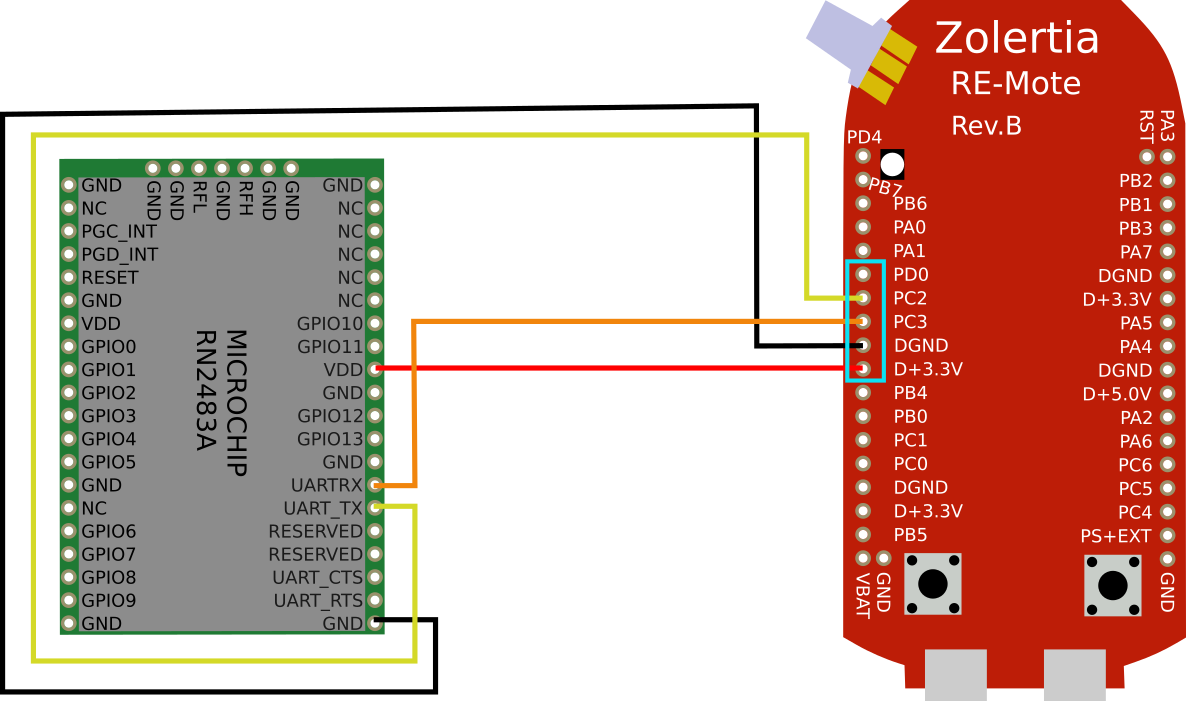
\includegraphics[scale=0.35]{res/pictures/montage.png}
        \caption{Schéma du raccordement du RN2483 au Re-Mote.}
        \label{fig:work-montage}
    \end{figure}

    Comme l'indique la table~\ref{table:work-pin-description} de description des pins, les pins PC2 et PC3 utilisés pour la connexion ne sont pas ceux défini pour l'usage d'une connexion UART. Ces pins sont choisis pour la connexion UART car ils sont accessibles à l'exterieur du boitier de la plateforme par un connecteur.
    
    Pour que la connexion UART avec le RN2483 soit possible via les pins choisis, des modifications 
    dans Contiki du fichier de configuration de la plateforme sont nécéssaires.
    Ainsi, les valeurs des macros suivantes ont été modifiées dans le fichier \texttt{arch/cpu/cc2538/cc2538-conf.h}:
    \begin{itemize}
        \item \texttt{UART1\_CONF\_BAUD\_RATE} est définie à $57600$ qui est le baudrate par défaut du RN2483
        \item \texttt{UART1\_RX\_PIN} est définie à $2$
        \item \texttt{UART1\_TX\_PIN} est définie à $3$
    \end{itemize}

    Comme pour l'implémentation de la racine LoRa, celle de la racine RPL est réalisée en 3 couches.
    qui sont intégrées dans Contiki comme un service. C'est à dire que le code des 3 couches se trouve dans le répertoire suivant: \texttt{os/services/loramac}.
    
    \begin{table}[H]
        \centering
        \makebox[\textwidth]{%
        \begin{tabular}{|l|l|l|l|}
        \hline
        \rowcolor[HTML]{C0C0C0} 
        Pin & Default name       & MC  & Description                                                                            \\ \hline
        4   & UART0.RX           & PA0 & Connected to the CP2104 USB-to-serial converter                                        \\ \hline
        5   & UART0.TX           & PA1 & Connected to the CP2104 USB-to-serial converter                                        \\ \hline
        6   & GPD0/I2C.Interrupt & PD0 & Generic pin, may be used as auxiliary pin for I2C/SPI                                  \\ \hline
        7   & I2C.SDA            & PC2 & \multicolumn{1}{p{10cm}|}{GPIO 20 mA output capability, pull-up. Shared with the RTCC and on-board low-power PIC} \\ \hline
        8   & I2C.SCL            & PC3 &  \multicolumn{1}{p{10cm}|}{GPIO 20 mA output capability, pull-up. Shared with the RTCC and on-board low-power PIC} \\ \hline
        9   & DGND               & N/A & Digital Ground                                                                         \\ \hline
        10  & D+3.3              & N/A & 3.3VDC output pin                                                                      \\ \hline
        11  & CC1200.GPIO0       & PB4 &  \multicolumn{1}{p{10cm}|}{CC1200 GPIO0 pin. If RF switch disables sub-GHz is available for other purposes}        \\ \hline
        12  & CC1200.GPIO2       & PB0 &  \multicolumn{1}{p{10cm}|}{CC1200 GPIO2 pin. If RF switch disables sub-GHz is available for other purposes}        \\ \hline
        13  & UART1.RX           & PC1 &  \multicolumn{1}{p{10cm}|}{GPIO 20 mA output capability, no pull-up or pull-down.}                                 \\ \hline
        14  & UART1.TX           & PC0 &  \multicolumn{1}{p{10cm}|}{GPIO 20 mA output capability, no pull-up or pull-down.  }                               \\ \hline
        \end{tabular}%
        }
        \caption{Extrait de la table de descrition des pins~\cite{zolertia-remote:datasheet}.}
        \label{table:work-pin-description}
        \end{table}
\newpage
\subsection*{Couche physique}
    Comme pour la racine LoRa, la couche physique définit les trame et les adresses LoRaMAC et sert 
    de driver pour le RN2483. La réception et l'envoi de trames UART est réalisée par deux 
    processus.

    Le processus de récéption permet d'éviter que le reste du code soit interrompu par une trame 
    UART entrante. Le code suivant illustre la déclaration de processus dans contiki.  

    \begin{minted}[linenos]{c}
PROCESS_THREAD(ph_rx, ev, data){
    PROCESS_BEGIN();
    /* UART configuration */
    uart_init(UART);
    uart_set_input(UART, &uart_rx);
    PROCESS_END();
}
    \end{minted}
    Tout ce qui se trouve entre les instructions des lignes 2 et 6 dépend du processus. Ainsi, la 
    fonction, \texttt{uart\_rx} qui traite les trames UART entrantes dépend bien de ce processus.
    Le rôle de cette fonction est d'accumuler tous les caractères d'une trame UART pour ensuite 
    appeler une fonction qui traîte cette trame. Elle supprime également les caractères ayant comme 
    valeur entière 254, 248, 192 et 240. Ces caractèrent apparaissent lors de certaines réponses 
    UART et perturbe la reconstruction de la trame. La cause de l'apparition de ces caractères 
    n'est pas identifiée.

    Une fois la trame UART assemblée, une fonction suivante vérifie si cette réponse est une 
    réponse attendue pour la trame précédemment envoyée. Si c'est le cas, elle envoie un évènement 
    qu'attend le processus d'envoi pour envoyer la prochaine trame UART. Si la trame UART reçue 
    contient la commande \textit{"radio\_rx"}, la fonction construit une trame LoRaMAC et l'envoie 
    à la couche supérieure.

    Le processus d'envoi apour rôle d'envoyer toutes les trames UART présentes dans le buffer 
    d'envoi. Il peut être bloqué si le buffer d'envoi est vide ou s'il attend une réponse à la 
    dernière trame envoyée. Si le buffer d'envoi est vide, le processus sera débloqué par la 
    réception de l'évènement \texttt{new\_tx\_frame\_event}, et s'il attend une réponse, il sera 
    débloqué par la réception de l'évènement \texttt{can\_send\_event}.

    Dans Contiki, les évènements sont créés et envoyé de la manière suivante:
    \begin{minted}[linenos]{c}
        process_event_t new_tx_frame_event = process_alloc_event();
        process_post(&ph_tx, new_tx_frame_event, NULL);
    \end{minted}
    
    Le type type \texttt{process\_event\_t} est en réalité un \texttt{unsigned char} qui est incrémenté à chaque appel de \texttt{process\_alloc\_event()}.

    Les fonctions publiques de la couche physique sont les suivantes:
    \begin{itemize}
        \item \textbf{\texttt{void phy\_init()}}\\
            Initialise la couche physique. C'est à dire, alloue les évènements, démarre les 
            processus et envoie les trames UART permettant de mettre en pause LoRaWAN et de définir 
            les paramètres de la radio.
        \item \textbf{\texttt{void phy\_register\_listener(int (* listener)(lora\_frame\_t frame)})}\\
            Enregistre la fonction callback qui sera appelée lorsqu'une trame LoRaMAC est reçue.
        \item \textbf{\texttt{int phy\_tx(lora\_frame\_t frame)}}\\
            Envoie une trame LoRaMAC.
        \item \textbf{\texttt{int phy\_timeout(int timeout)}}\\
            Définis le temps d'expiration du watchdog timer.
        \item \textbf{\texttt{int phy\_sleep(int duration)}}\\
            Met le RN2483 en mode sommeil.
        \item \textbf{\texttt{int phy\_rx()}}\\
            Met le RN2483 en mode réception.
    \end{itemize}

    Toues ces fonctions créent une trame UART qu'elle ajoute au buffer d'envoi.

\subsection*{Couche MAC}
    La couche MAC définit 3 états: \textsc{alone}, \textsc{ready} et \textsc{wait\_response}.
    Ces états correspondent à ceux défini dans la section~\ref{sec:archi-loramac:proto}, mis à part l'état \textsc{sleep} qui n'a pas 
    besoin d'être défini explicitement, car dans cet état, le noeud attend, et donc rien d'autre ne peut se 
    passer. En effet, comme le noeud ne peut basculer dans cet état que si le transmission d'une 
    trame JOIN a échouée (i.e. après trois retransmissions), et qu'aucune trame LoRaMAC ne peut être reçue il impossible qu'il bascule dans cet état.
    De plus, aucune trame ne peut être envoyée, car tant que le noeud n'a pas rejoint le réseau LoRaMAC, 
    la radio 802.15.4 et le protocole de routage RPL ne sont pas actifs.
    Le premier état est l'état initiale, le second est utilisé quand la racine RPL est prête à 
    envoyer une trame et le dernier est utilisé quand elle attend une réponse à une trame envoyée.

    Cette implémentation utilise un processus qui envoi les trames disponibles dans un buffer. 
    Ce processus peut être bloqué si le buffer est vide ou si l'état est différent de \textsc{ready}. Il peut être débloqué respectivement par les évènements
    \texttt{new\_tx\_frame\_event} et \texttt{state\_change\_event}. Ce processus démarre également un timer, \texttt{retransmit\_timer} lorsqu'une trame attend une réponse en retour. C'est à dire, lorsqu'il envoie une trame QUERY ou une trame avec le flag k à \textit{true}.
    
    Comme pour l'implémentation de la racine LoRa, une fois que la fonction qui réceptionne une trame a vérifié par l'adresse de destination, que la trame est destinée à un noeud de son réseau RPL ou à elle même, elle va envoyer cette trame vers la fonction appropriée.

    \subsubsection*{Réception d'une trame JOIN\_RESPONSE}
        La trame est considérée comme valide si les conditions suivantes sont vérifiées:
        \begin{itemize}
            \item L'état MAC est \textsc{alone}
            \item L'adresse de destination est celle de la racine RPL
            \item La taille du payload est 2 ( taille de la chaîne de caractères hexadecimal du préfixe d'un octet)
            \item le numéro de séquence de la trame est 0
        \end{itemize}

        Si la trame n'est pas valide elle est ignorée. En revanche, si elle est valide, l'état est changé à \textsc{ready}, la processus d'envoi est démarré et la racine RPL met à jour son adresse. En effet, pour l'envoi de la trame JOIN la racine RPL n'ayant pas encore de préfixe, son préfixe était les huit bits de poids fort de son \textit{node-id}. En plus de ces actions, un timer
        \texttt{query\_timer} servant à envoyer periodiquement une trame QUERY est démarré, et l'évènement \texttt{loramac\_network\_joined} est envoyé à tous les processus.


    \subsubsection*{Réception d'une trame ACK}
        Si le numéro de séquence de la trame est différent à celui de la dernière trame envoyée, elle est ignorée. Sinon, les actions suivantes sont éffectuées:
        \begin{itemize}
            \item le timer \texttt{retransmit\_timer} est stoppé
            \item si la dernière trame envoyée était une QUERY, le timer \texttt{query\_timer} est redémarré
            \item l'état est changé à READY et le processus d'envoi est prévenu du changement d'état
        \end{itemize}

    \subsubsection*{Réception d'une trame DATA}
        Si $sf<se$, la trame est ignorée. Sinon elle est traitée. Si $sf > se$, cela signifie que $sf - se$ trames ont été perdues. Ensuite la trame est envoyée à la couche supérieure.

        Si la flag \textit{next} est à \textit{true}, cela signifie que d'autres trames vont être reçues. Donc, la racine RPL se met en mode écoute et redémarre le timer \texttt{retransmit\_timer}. Sinon, le timer \texttt{query\_timer} est redémarré, l'état est changé à \textsc{ready} et le processus d'envoi est prévenu de ce changement.

    \subsubsection*{Expiration du timer \texttt{retransmit\_timer}}
        A l'expiration de ce timer, si le nombre de retransmissions n'a pas atteint son maximum 
        défini par la macro \texttt{MAX\_RETRANSMIT}, la dernière trame envoyée est retransmissions.
        Sinon l'envoi de la dernière trame est considéré comme échoué et l'état est changé à \textsc
        {ready} sauf si la trame qui n'a pas pu être envoyée est trame JOIN. Dans ce cas, le temps 
        d'expiration du timer est allongé comme décrit par l'équation~\ref{eq:archi-wait}.

    \subsubsection*{Fonctions publiques}
        Les fonctions publiques utilisable par les autres couches sont les suivantes:
        \begin{itemize}
            \item \textbf{\texttt{void mac\_root\_start()}}\\
                Initialise le protocole LoRaMAC. C'est à dire, défini l'adresse du noeud, l'état 
                initiale, crée les évènements, initialise la couche physique, envoie une trame 
                JOIN, met la radio en mode réception et active le \texttt{retransmit\_timer}.

            \item \textbf{\texttt{int mac\_send\_packet(lora\_addr\_t src\_addr, bool need\_ack, void* data)}}\\
                Permet d'envoyer un paquet à l'adresse de destination. Si le paramètre \texttt{need\_ack} est à \textit{true}, un aquitement sera demandé pour la trame envoyée.

            \item \textbf{\texttt{void loramac\_set\_input\_callback(void (* listener)(lora\_addr\_t *src, lora\_addr\_t *dest, char* data))}}\\
                Permet d'enregistrer une fonction callback qui sera appelée quand un paquet est disponible.
        \end{itemize}

\subsection*{Couche IP}
    Ce qui est appelé la couche IP est une interface entre le protocole LoRaMAC et la stack TCP/IP de Contiki. Les paquets destinés à une adresse pour lesquels aucune route n'est trouvée sont récupérer par une interface définie comme suit dans le fichier \texttt{os/net/ipv6/uip.h}.
    \begin{minted}[linenos]{c}
struct uip_fallback_interface {
  void (*init)(void);
  /**
   * \retval >=0
   *         in case of success
   * \retval <0
   *         in case of failure
   */
  int (*output)(void);
};
    \end{minted}
    Cette interface doit être la valeur d'une macro \texttt{UIP\_FALLBACK\_INTERFACE} qui pour ce projet est définie dans \texttt{module-macros.h} présent dans le service \texttt{loramac}.
    Ainsi, quand un paquet IPv6 est destiné à une adresse pour laquelle aucune route n'est trouvée, la fonction  \texttt{output()} de l'interface est appelée.

    L'utilisation de cette interface a été choisie car il n'estactuellement pas possible d'utiliser deux interfaces réseaux dans Contiki. C'est donc le seul moyen trouvé pour récupérer les paquets destinés à une adresses externe au réseau RPL.

    Contiki possède un buffer, le buffer uIP, qui est utilisé pour stocker les paquets entrants et sortants.
    L'accès à ce buffer se fait via la macro \texttt{uip\_buf} définie dans le même fichier que la structure \texttt{uip\_fallback\_interface}. Une autre macro de Contiki utilisée dans l'interface est la macro \texttt{uip\_len} qui est la longueur d'un paquet disponible dans le buffer. Enfin, Contiki fourni des macros faciliant l'accès au buffer uIP comme la macro \texttt{UIP\_IP\_BUF} qui permet d'accèder directement au header IPv6. Le header Ipv6 est défini comme suit:
    \begin{minted}[linenos]{c}
struct uip_ip_hdr {
  /* IPV6 header */
  uint8_t vtc;
  uint8_t tcflow;
  uint16_t flow;
  uint8_t len[2];
  uint8_t proto, ttl;
  uip_ip6addr_t srcipaddr, destipaddr;
};
    \end{minted}

    Le code suivant est celui de la fonction \texttt{output} de l'interface.

    \begin{minted}[linenos]{c}
static int output(void){ 
  static char data[(UIP_CONF_BUFFER_SIZE-32)*2];
  int uip_index = 0;
  int data_index = 0;
  
  while(uip_index<uip_len){
    if(uip_index==8){
      // skip src and dest ipv6 addr
      uip_index= UIP_IPH_LEN; // UIP_IPH_LEN is the ipv6 header size
    }

    sprintf(data+data_index, "%02X", uip_buf[uip_index]);
    data_index+=2;
    uip_index++;
  }

  lora_addr_t src_addr;
  ipv62lora(&(UIP_IP_BUF->srcipaddr), &src_addr);//convert src address
  mac_send_packet(src_addr, true, &data);
  return 0;
}
    \end{minted}
    A la ligne 1, le tableau de caractère contenant la payload de la trame LoRaMAC est défini. Sa 
    taille est \texttt{(UIP\_CONF\_BUFFER\_SIZE-32)*2}. La macro \texttt{UIP\_CONF\_BUFFER} défini 
    la taille du buffer uIP. Cette macro est définie dans \texttt{contiki-default-conf.h}. Pour ce 
    projet, sa valeur initiale de 1280 a été modifiée à 279. Cette taille est 247, la 
    taille de la payload d'une trame LoRaMAC à laquelle on a ajouté 32 octets qui est la taille des 
    deux adresses Ipv6 (source et destination) car celles-ci ne se retrouvent pas dans une trame LoRaMAC.
    A la taille du buffer uIP, la taille des deux adresses IPv6 est soustraite car elles ne se 
    trouvent pas dans la payload de la trame LoRaMAC. Ensuite cette taille est mutlipliée par deux 
    car il faut deux caractères hexadecimal pour représenter un octet.

    Ensuite la boucle de la ligne 6 parcourt le buffer uIP et convertit chaque octet en hexadecimal.
    A la fin de cette boucle l'adresse source est convertie en adresse LoRaMAC comme défini dans la solution retenue de la section~\ref{sec:archi-adresses}. Enfin, l'adresse source et la payload sont envoyées à la couche LoRaMAC.

    Lorsqu'une trame LoRaMAC est reçue la fonction callback enregistré auprès de la couche LoRaMAC 
    convertit les adresses LoRaMAC source et destination en adresses IPv6, écrit les 8 
    octets de poids fort du header dans le buffer uIP et écrit les adresses converties dans ce buffer avant d'écrire la payload de la trame LoRaMAC.

    La fonction \texttt{init} de l'interface démarre un processus. Ce processus désactive la radio, 
    initialise la couche MAC et attend l'évènement\\ \texttt{loramac\_network\_joined}. Une fois cet 
    évènement reçu, ce process défini le préfixe IPv6 qui sera diffusé dans le réseau RPL, allume 
    la radio et démarre le protocole de routage.

%\subsection*{Discussion}
%\todo{todo}
%premiere idée: implémenter niveau app
%pourquoi les buffers
%moyen de les supprimer


    % Please add the following required packages to your document preamble:
% \usepackage{graphicx}
% \usepackage[table,xcdraw]{xcolor}
% If you use beamer only pass "xcolor=table" option, i.e. \documentclass[xcolor=table]{beamer}
